\documentclass{ximera}

\usepackage{epsfig}

\graphicspath{
  {./}
  {figures/}
}


\usepackage{morewrites}

%\newcounter{ccounter}
%\setcounter{ccounter}{1}
%\newcommand{\Chapter}[1]{\setcounter{chapter}{\arabic{ccounter}}\chapter{#1}\addtocounter{ccounter}{1}}

%\newcommand{\section}[1]{\section{#1}\setcounter{thm}{0}\setcounter{equation}{0}}

%\renewcommand{\theequation}{\arabic{chapter}.\arabic{section}.\arabic{equation}}
%\renewcommand{\thefigure}{\arabic{chapter}.\arabic{figure}}
%\renewcommand{\thetable}{\arabic{chapter}.\arabic{table}}

%\newcommand{\Sec}[2]{\section{#1}\markright{\arabic{ccounter}.\arabic{section}.#2}\setcounter{equation}{0}\setcounter{thm}{0}\setcounter{figure}{0}}

\newcommand{\Sec}[2]{\section{#1}}

\setcounter{secnumdepth}{2}
%\setcounter{secnumdepth}{1} 

%\newcounter{THM}
%\renewcommand{\theTHM}{\arabic{chapter}.\arabic{section}}

\newcommand{\trademark}{{R\!\!\!\!\!\bigcirc}}
%\newtheorem{exercise}{}

\newcommand{\dfield}{{\sf dfield9}}
\newcommand{\pplane}{{\sf pplane9}}

\newcommand{\EXER}{\section*{Exercises}}%\vspace*{0.2in}\hrule\small\setcounter{exercise}{0}}
\newcommand{\CEXER}{}%\vspace{0.08in}\begin{center}Computer Exercises\end{center}}
\newcommand{\TEXER}{} %\vspace{0.08in}\begin{center}Hand Exercises\end{center}}
\newcommand{\AEXER}{} %\vspace{0.08in}\begin{center}Hand Exercises\end{center}}

% BADBAD: \newcommand{\Bbb}{\bf}

\newcommand{\R}{\mbox{$\Bbb{R}$}}
\newcommand{\C}{\mbox{$\Bbb{C}$}}
\newcommand{\Z}{\mbox{$\Bbb{Z}$}}
\newcommand{\N}{\mbox{$\Bbb{N}$}}
\newcommand{\D}{\mbox{{\bf D}}}
\usepackage{amssymb}
%\newcommand{\qed}{\hfill\mbox{\raggedright$\square$} \vspace{1ex}}
%\newcommand{\proof}{\noindent {\bf Proof:} \hspace{0.1in}}

\newcommand{\setmin}{\;\mbox{--}\;}
\newcommand{\Matlab}{{M\small{AT\-LAB}} }
\newcommand{\Matlabp}{{M\small{AT\-LAB}}}
\newcommand{\computer}{\Matlab Instructions}
\newcommand{\half}{\mbox{$\frac{1}{2}$}}
\newcommand{\compose}{\raisebox{.15ex}{\mbox{{\scriptsize$\circ$}}}}
\newcommand{\AND}{\quad\mbox{and}\quad}
\newcommand{\vect}[2]{\left(\begin{array}{c} #1_1 \\ \vdots \\
 #1_{#2}\end{array}\right)}
\newcommand{\mattwo}[4]{\left(\begin{array}{rr} #1 & #2\\ #3
&#4\end{array}\right)}
\newcommand{\mattwoc}[4]{\left(\begin{array}{cc} #1 & #2\\ #3
&#4\end{array}\right)}
\newcommand{\vectwo}[2]{\left(\begin{array}{r} #1 \\ #2\end{array}\right)}
\newcommand{\vectwoc}[2]{\left(\begin{array}{c} #1 \\ #2\end{array}\right)}



\newcommand{\inv}{^{-1}}
\newcommand{\CC}{{\cal C}}
\newcommand{\CCone}{\CC^1}
\newcommand{\Span}{{\rm span}}
\newcommand{\rank}{{\rm rank}}
\newcommand{\trace}{{\rm tr}}
\newcommand{\RE}{{\rm Re}}
\newcommand{\IM}{{\rm Im}}
\newcommand{\nulls}{{\rm null\;space}}

\newcommand{\dps}{\displaystyle}
\newcommand{\arraystart}{\renewcommand{\arraystretch}{1.8}}
\newcommand{\arrayfinish}{\renewcommand{\arraystretch}{1.2}}
\newcommand{\Start}[1]{\vspace{0.08in}\noindent {\bf Section~\ref{#1}}}
\newcommand{\exer}[1]{\noindent {\bf \ref{#1}}}
\newcommand{\ans}{}
\newcommand{\matthree}[9]{\left(\begin{array}{rrr} #1 & #2 & #3 \\ #4 & #5 & #6
\\ #7 & #8 & #9\end{array}\right)}
\newcommand{\cvectwo}[2]{\left(\begin{array}{c} #1 \\ #2\end{array}\right)}
\newcommand{\cmatthree}[9]{\left(\begin{array}{ccc} #1 & #2 & #3 \\ #4 & #5 &
#6 \\ #7 & #8 & #9\end{array}\right)}
\newcommand{\vecthree}[3]{\left(\begin{array}{r} #1 \\ #2 \\
#3\end{array}\right)}
\newcommand{\cvecthree}[3]{\left(\begin{array}{c} #1 \\ #2 \\
#3\end{array}\right)}
\newcommand{\cmattwo}[4]{\left(\begin{array}{cc} #1 & #2\\ #3
&#4\end{array}\right)}

\newcommand{\Matrix}[1]{\ensuremath{\left(\begin{array}{rrrrrrrrrrrrrrrrrr} #1 \end{array}\right)}}

\newcommand{\Matrixc}[1]{\ensuremath{\left(\begin{array}{cccccccccccc} #1 \end{array}\right)}}



\renewcommand{\labelenumi}{\theenumi)}
\newenvironment{enumeratea}%
{\begingroup
 \renewcommand{\theenumi}{\alph{enumi}}
 \renewcommand{\labelenumi}{(\theenumi)}
 \begin{enumerate}}
 {\end{enumerate}\endgroup}



\newcounter{help}
\renewcommand{\thehelp}{\thesection.\arabic{equation}}

%\newenvironment{equation*}%
%{\renewcommand\endequation{\eqno (\theequation)* $$}%
%   \begin{equation}}%
%   {\end{equation}\renewcommand\endequation{\eqno \@eqnnum
%$$\global\@ignoretrue}}

%\input{psfig.tex}

\author{Martin Golubitsky and Michael Dellnitz}

%\newenvironment{matlabEquation}%
%{\renewcommand\endequation{\eqno (\theequation*) $$}%
%   \begin{equation}}%
%   {\end{equation}\renewcommand\endequation{\eqno \@eqnnum
% $$\global\@ignoretrue}}

\newcommand{\soln}{\textbf{Solution:} }
\newcommand{\exercap}[1]{\centerline{Figure~\ref{#1}}}
\newcommand{\exercaptwo}[1]{\centerline{Figure~\ref{#1}a\hspace{2.1in}
Figure~\ref{#1}b}}
\newcommand{\exercapthree}[1]{\centerline{Figure~\ref{#1}a\hspace{1.2in}
Figure~\ref{#1}b\hspace{1.2in}Figure~\ref{#1}c}}
\newcommand{\para}{\hspace{0.4in}}

\renewenvironment{solution}{\suppress}{\endsuppress}

\ifxake
\newenvironment{matlabEquation}{\begin{equation}}{\end{equation}}
\else
\newenvironment{matlabEquation}%
{\let\oldtheequation\theequation\renewcommand{\theequation}{\oldtheequation*}\begin{equation}}%
  {\end{equation}\let\theequation\oldtheequation}
\fi

\makeatother


\title{m7.tex}

\begin{document}
\begin{abstract}
BADBAD
\end{abstract}
\maketitle

\chapter{Qualitative Theory of Planar ODEs}

\subsection*{Section~\protect{\ref{S:6.7}} Sinks, Saddles, and Sources}
\rhead{S:6.7}{SINKS, SADDLES, AND SOURCES}

\exer{E:stabmata} \ans The origin is not asymptotically stable.

\soln Theorem~\ref{C:asympstlin} states that the origin is a stable
equilibrium only if all eigenvectors have negative real part.  The
characteristic polynomial of $C$ is $p_C(\lambda) = \lambda^2 - 2\lambda
- 5$.  Thus, the eigenvalues are $\lambda_1 = 1 + \sqrt{6}$ and
$\lambda_2 = 1 - \sqrt{6}$. Since $\lambda_1 > 0$, the origin
is not stable.

\exer{E:stabmatb} \ans The origin is asymptotically stable.

\soln The characteristic polynomial of the matrix is $p_C(\lambda) =
\lambda^2 + 2\lambda + 7$.  Thus, the eigenvalues are $\lambda_1 =
-1 + 2\sqrt{2}i$ and $\lambda_2 = -1 - 2\sqrt{2}i$.  Both of these
have negative real part, so the origin is stable.

\exer{E:stabmatc} \ans The origin is not asymptotically stable.

\soln The characteristic polynomial of the matrix is $p_C(\lambda) =
\lambda^2 - 3\lambda - 11$.  Thus, the eigenvalues are $\lambda_1 =
\frac{3}{2} + \sqrt{53}$ and $\lambda_2 = \frac{3}{2} - \sqrt{53}$.
Since $\lambda_1 > 0$, the origin is not stable.

\exer{E:sisasoa} \ans The origin of the system $\dot{X} = CX$ is a sink.

\soln The characteristic polynomial of $C$ is
$p_C(\lambda) = \lambda^2 + 3\lambda + 2$.  So the eigenvalues are
$\lambda_1 = -1$ and $\lambda_2 = -2$.  Since both eigenvalues have
negative real part, the origin is a sink.

\exer{E:sisasob} \ans The origin of the system $\dot{X} = CX$ is a saddle.

\soln The characteristic polynomial of $C$ is
$p_C(\lambda) = \lambda^2 - \lambda - 6$.  So the eigenvalues are
$\lambda_1 = 3$ and $\lambda_2 = -2$.  Since one eigenvalue is negative
and one is positive, the origin is a saddle.

\exer{E:sisasoc} \ans The origin of the system $\dot{X} = CX$ is a source.

\soln The characteristic polynomial of $C$ is
$p_C(\lambda) = \lambda^2 - 6\lambda + 10$.  So the eigenvalues are
$\lambda = 3 \pm i$.  Since both eigenvalues have positive real part,
the origin is a source.

\exer{E:sisasod} \ans The origin of the system $\dot{X} = CX$ is a source.

\soln The characteristic polynomial of $C$ is
$p_C(\lambda) = \lambda^2 - 11\lambda + 24$.  So the eigenvalues are
$\lambda_1 = 8$ and $\lambda_2 = 3$.  Since both eigenvalues have
positive real part, the origin is a source.

\exer{E:sisasoe} \ans The origin of the system $\dot{X} = CX$ is a saddle.

\soln The characteristic polynomial of $C$ is
$p_C(\lambda) = \lambda^2 - 18\lambda - 40$.  So the eigenvalues are
$\lambda_1 = 20$ and $\lambda_2 = -2$.  Since one eigenvalue is positive
and one is negative, the origin is a saddle.

\exer{E:sisasof} \ans The origin of the system $\dot{X} = CX$ is a source.

\soln The characteristic polynomial of $C$ is
$p_C(\lambda) = \lambda^2 - 2\lambda + 17$.  So the eigenvalues are
$\lambda = 1 \pm 4i$.  Since both eigenvalues have positive real part,
the origin is a source.

\exer{E:sssa} \ans The origin is a source.

\soln Enter the system into {\tt pplane5}.  Then compute trajectories with
different initial conditions and note that all trajectories go away from
the origin in forward time.

\exer{E:sssb} \ans The origin is a saddle.

\soln Enter the system into {\tt pplane5}.  Then compute trajectories with
different initial conditions and note that some trajectories approach the
origin in forward time, while some approach the origin in backward time.

\exer{E:sssc} \ans The origin is a saddle.

\soln Enter the system into {\tt pplane5}.  Then compute trajectories with
different initial conditions and note that some trajectories approach the
origin in forward time, while some approach the origin in backward time.

\exer{E:sssd} \ans The origin is a sink.

\soln Enter the system into {\tt pplane5}.  Then compute trajectories with
different initial conditions and note that all trajectories approach
the origin in forward time.


\exer{E:sima}
(a) \ans
\[
P = \frac{\sqrt{2}}{2}\mattwo{1}{-1}{1}{1}.
\]
The matrix $P$ rotates vectors in the plane by $45^\circ$ counterclockwise.

\soln Enter matrices $B$ and $C$ into \Matlabp.  Then type
\begin{verbatim}
[Q,D] = eig(C);
\end{verbatim}
Since $C$ has distinct eigenvalues (you can check this using
\Matlabp), the matrix $D$ is a diagonal matrix with the eigenvalues of
$C$ along its diagonal.  This matrix is similar to $C$.  Indeed, $D =
Q^{-1}CQ$.  The matrix $D$ is also similar to $B$, and $D= R^{-1}BR$.
Find the matrix $R$ by typing
\begin{verbatim}
[R,D] = eig(B);
\end{verbatim}
We know that $D = R^{-1}BR$ and $D = Q^{-1}CQ$ for the same diagonal
matrix $D$.  Therefore,
\[
B = RDR^{-1} = R(Q^{-1}CQ)R^{-1} = (QR^{-1})^{-1}C(QR).
\]
Thus, $P = QR^{-1}$, and typing
\begin{verbatim}
P = Q*inv(R)
\end{verbatim}
in \Matlab yields $P$.

(b) \ans The solutions of $\dot{X} = CX$ are found by rotating the
solutions of $\dot{X} = BX$ by $45^\circ$ counterclockwise.

\soln Enter the system $\dot{X} = BX$ into {\tt pplane5}.  Then enter the
system $\dot{X} = CX$.  Note that both systems are saddles.  You can
plot the stable and unstable trajectories at the origin in each system
to see that the trajectories for $\dot{X} = CX$ appear to be about
$45^\circ$ counterclockwise of those for $\dot{X} = BX$.  Thus, if
$X(t)$ is a solution to $\dot{X} = BX$, then $PX(t)$ is a solution to
$\dot{X} = CX$, verifying Lemma~\ref{L:simsoln}.

\exer{E:simb}
(a) \ans
\[
P \approx \mattwo{7.1063}{0}{0}{0.7106}.
\]
The matrix $P$ stretches the $x$-coordinate of a vector and shrinks the
$y$-coordinate.

\soln Enter matrices $B$ and $C$ into \Matlabp.  Then type
\begin{verbatim}
[Q,D] = eig(C);
\end{verbatim}
Since $C$ has distinct eigenvalues (you can check this using
\Matlabp), the matrix $D$ is a diagonal matrix with the eigenvalues of
$C$ along its diagonal.  This matrix is similar to $C$.  Indeed, $D =
Q^{-1}CQ$.  The matrix $D$ is also similar to $B$, and $D= R^{-1}BR$.
Find the matrix $R$ by typing
\begin{verbatim}
[R,D] = eig(B);
\end{verbatim}
We know that $D = R^{-1}BR$ and $D = Q^{-1}CQ$ for the same diagonal
matrix $D$.  Therefore,
\[
B = RDR^{-1} = R(Q^{-1}CQ)R^{-1} = (QR^{-1})^{-1}C(QR).
\]
Thus, $P = QR^{-1}$, and typing
\begin{verbatim}
P = Q*inv(R)
\end{verbatim}
in \Matlab yields $P$.

(b) \ans The solutions of $\dot{X} = CX$ are obtained from the solutions
of $\dot{X} = BX$ by stretching the $x$-coordinate by a factor of $7.1063$
and the $y$-coordinate by a factor of $0.7106$.

\soln Enter the system $\dot{X} = BX$ into {\tt pplane5}.  Then enter the
system $\dot{X} = CX$.  Note that both systems are spirals.  You can
plot trajectories in each system to see that the trajectories for
$\dot{X} = CX$ appear to be similar to those for $\dot{X} = BX$, but
stretched in one direction and contracted in the other.  Thus, if
$X(t)$ is a solution to $\dot{X} = BX$, then $PX(t)$ is a solution to
$\dot{X} = CX$, verifying Lemma~\ref{L:simsoln}.



\subsection*{Section~\protect{\ref{S:PlanarSystems}} Phase Portraits of Sinks}
\rhead{S:PlanarSystems}{PHASE PORTRAITS OF SINKS}

\exer{c6.8.1a} \ans The origin is a saddle.

\soln Compute $\det(C) = -5$.  If the determinant of a matrix $C$ is
negative, the phase portrait of $\dot{X} = CX$ is a saddle.

\exer{c6.8.1b} \ans The origin is a spiral sink.

\soln First, compute $\det(C) = 9 > 0$ and $\trace(C) = -2 < 0$.  Thus,
the origin is a sink.  Since the discriminant is $D = 4 - 36 = -32 < 0$,
the origin is a spiral.

\exer{c6.8.1c} \ans The origin is a saddle.

\soln The determinant of the matrix is $\det(C) = -11 < 0$.

\exer{c6.8.2a}
\ans One possible solution is $C = \mattwo{1}{0}{3}{-1}$.

\soln Since the system has an invariant manifold in the direction $(2,3)$,
$v_1 = (2,3)$.  Let $\lambda_1$ be the eigenvalue associated to $v_1$.
Since the manifold is unstable, $\lambda_1 > 0$.  The requirement
that the system has a saddle at the origin implies that $C$ has a second
eigenvalue $\lambda_2 < 0$.  Choose a second eigenvector $v_2$ independent
of $v_1$, such as $v_2 = (0,1)$ and choose eigenvalues, for example:
$\lambda_1 = 1$ and $\lambda_2 = -1$.

\para The matrix $C$ has two real eigenvalues.  Thus, by
Theorem~\ref{T:putinform}, $C$ is similar
to the diagonal matrix $D$ which has $\lambda_1$ and $\lambda_2$ as
entries along the main diagonal.  Therefore, $C = PDP^{-1}$, where $P$
is the matrix whose columns are the eigenvectors of $C$.  Thus,
\[
C = \mattwo{2}{0}{3}{1}\mattwo{1}{0}{0}{-1}\mattwo{\frac{1}{2}}{0}
{-\frac{3}{2}}{1} = \mattwo{1}{0}{3}{-1}. \]

\exer{c6.8.2b}
\ans One possible matrix is $C = \mattwo{-0.5}{-1}{1}{-0.5}$.

\soln Since the origin is a spiral, the eigenvalues of $C$ are a complex
conjugate pair, $lambda_1 = \sigma + \tau i$ and $lambda_2 = \sigma -
\tau i$.  Since the origin is a sink, $\sigma$ is negative, and determines
the rate at which solutions decay to the origin, so $\sigma = -0.5$.
From Section~\ref{S:evchp}, we know that the matrix
\[ \mattwo{\sigma}{-\tau}{\tau}{\sigma} \]
has complex conjugate eigenvalues $\sigma \pm \tau$ if $\tau \neq 0$.
Thus, this matrix is a solution for any nonzero $\tau$.  For example,
let $\tau = 1$.

\exer{c6.8.2c}
\ans One possible matrix is $C = \mattwo{1}{0}{1}{1}$.

\soln Since the system has an improper nodal source at the origin, there
are two real equal positive eigenvalues, $\lambda_1 = \lambda_2 > 0$,
associated to a single eigenvector, $v$.  Let $\lambda = 1$ be an
eigenvalue.  The trajectories of an improper nodal system approach the
origin tangent to the eigenvector, so, since trajectories approach
tangent to the $y$-axis, the eigenvector is $v = (0,1)$.  By
Theorem~\ref{T:putinform}, if $C$ has one
real eigenvector, then $C = PDP^1$, where
\[ D = \mattwo{\lambda}{1}{0}{\lambda} \AND P = (v|w) \]
such that $Cv = v + \lambda w$.  We can assign an arbitrary value to
$w$.  For example, let $w = (1,0)$.  Then,
\[ C = \mattwo{0}{1}{1}{0}\mattwo{1}{1}{0}{1}\mattwo{0}{1}{1}{0} =
\mattwo{1}{0}{1}{1}. \]

\exer{c6.8.2d}
\ans One possible matrix is $C = \mattwo{-1}{0}{1}{-2}$.

\soln Since the system has a nodal sink, the eigenvalues are real, unequal
and negative.  That is, $\lambda_2 < \lambda_1 < 0$.  The trajectories
of a nodal system approach the origin tangent to the eigenvector
associated to the eigenvalue with smaller absolute value.  Thus, for
this system, $v_1 = (1,1)$ is an eigenvalue associated to $\lambda_1$.
Arbitrarily assign values to $\lambda_1$, $\lambda_2$ and $v_2$, with
the given restrictions.  For example, let $\lambda_1 = -1$, $\lambda_2
= -2$ and $v_2 = (0,1)$.  Therefore, by
Theorem~\ref{T:putinform}, $C = PDP^{-1}$, where
\[ D = \mattwo{-1}{0}{0}{-2} \AND P = (v_1|v_2). \]
Thus,
\[ C = \mattwo{1}{0}{1}{1}\mattwo{-1}{0}{0}{-2}\mattwo{1}{0}{-1}{1} =
\mattwo{-1}{0}{1}{-2}. \]

\exer{c6.8.3}
In the figure on the left, $x$ oscillates away from the origin as $t$
increases, so the origin is a spiral source.  Therefore, the eigenvalues
of $C$ are a complex conjugate pair with positive real part.

\para In the figure on the right, both $x$ and $y$ cross $0$, then
tend back towards $0$ from the opposite direction.  Therefore, the origin
is an improper nodal sink, so the eigenvalues are real, equal and
negative, and there is one independent eigenvector.

\exer{c6.8.4a}
(a) As $t$ increases, solutions tend away from the origin, so the origin
is not asymptotically stable.

(b) Figure~\ref{c6.8.4a} shows that this system is a nodal source,
thus has two real eigenvectors.

\exer{c6.8.4b}
(a) As $t$ increases, solutions tend away from the origin, so the origin
is not asymptotically stable.

(b) Figure~\ref{c6.8.4b} shows that this system is a saddle, and thus
has two real eigenvectors.

\begin{figure}[htb]
                       \centerline{%
                       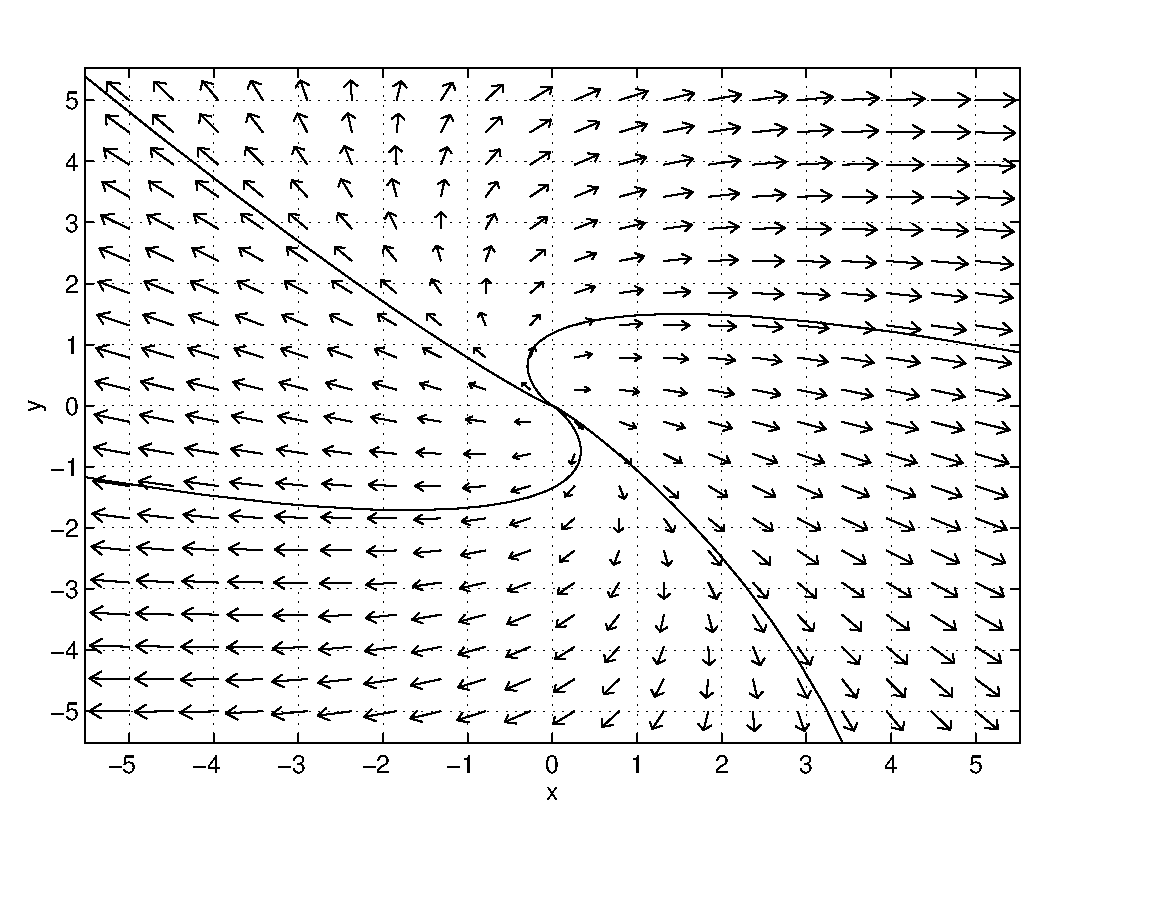
\psfig{file=exfigure/6-8-4a.eps,width=2.75in}
                       \psfig{file=exfigure/6-8-4b.eps,width=2.75in}}
                \centerline{Figure~\ref{c6.8.4a}\hspace{2.1in}
Figure~\ref{c6.8.4b}}
\end{figure}


\subsection*{Section~\protect{\ref{S:6.9}} Phase Portraits of Nonhyperbolic
Systems}
\rhead{S:6.9}{PHASE PORTRAITS OF NONHYPERBOLIC SYSTEMS}

\exer{c6.9.1a} \ans One such matrix is $C = \mattwo{0}{-1}{1}{0}$.

\soln More generally, for any matrix
\[
C = \mattwo{\sigma}{-\tau}{\tau}{\sigma}
\]
such that $\sigma = 0$ and $\tau \neq 0$, the differential equation
$\dot{X} = CX$ will have the origin as a center.

\exer{c6.9.1b} \ans One such matrix is $C = \mattwo{0}{0}{2}{1}$.

\soln Saddle nodes are generated by systems with eigenvalues $\lambda_1
= 0$ and $\lambda_2 \neq 0$.  All trajectories converge on the
eigenvector associated to eigenvalue $0$, so $v_1 = (-1,2)$ is the
eigenvector associated to $\lambda_1$.  Let $v_2 = (0,1)$ be the
eigenvector associated to $\lambda_2$, and let $\lambda_2 = 1$.  Then,
according to Theorem~\ref{T:putinform}, $C
= PDP^{-1}$, where $D$ is the diagonal matrix will $\lambda_1$ and
$\lambda_2$ along the main diagonal, and $P = (v_1|v_2)$.  Thus,
\[
C = \mattwo{-1}{0}{2}{1}\mattwo{0}{0}{0}{1}\mattwo{-1}{0}{2}{1}
= \mattwo{0}{0}{2}{1}.
\]

\exer{c6.9.2}
Three trajectories of the undamped equation are shown in Figure~\ref{c6.9.2}a,
and one trajectory of the damped equation is shown in Figure~\ref{c6.9.2}b.

%(a) \ans The first order linear system corresponding to \Ref{ex:uspring} is
%\[ \begin{array}{rcl}
%\dot{x} & = & y \\
%\dot{y} & = & -\kappa x. \end{array}
%\]
%\soln  The equation \Ref{ex:uspring} is a special case of \Ref{E:2ndorder}
%in which $a(x) = 0$ and $b(x) = \kappa$.

%(b) \ans The damped first order linear system is
%\[ \begin{array}{rcl}
%\dot{x} & = & y \\
%\dot{y} & = & -\kappa x -\sigma y. \end{array}
%\]
%\soln When friction is taken into account, the second order
%differential equation is
%\[ \frac{d^2x}{dt^2} + \sigma\frac{dx}{dt} + \kappa x = 0, \]
%which is also a special case of \Ref{E:2ndorder}.  In this case,
%$a(x) = \sigma$ and $b(x) = \kappa$.

%(c) The three sample trajectories for the solution to the
%frictionless system (Figure \ref{c3.5.6}a) are ellipses
%around the origin.  This makes sense, since $|x|$ (the distance
%of the spring from its natural position) is at a maximum when
%$|y|$ (the speed of the spring's motion) is $0$.  The sample
%trajectory for the damped system (Figure \ref{c3.5.6}b) 
%is a spiral, since friction
%both slows the spring and shortens the distance of motion until
%the spring comes to rest at its natural length.

\begin{figure}[htb]
                       \centerline{%
                       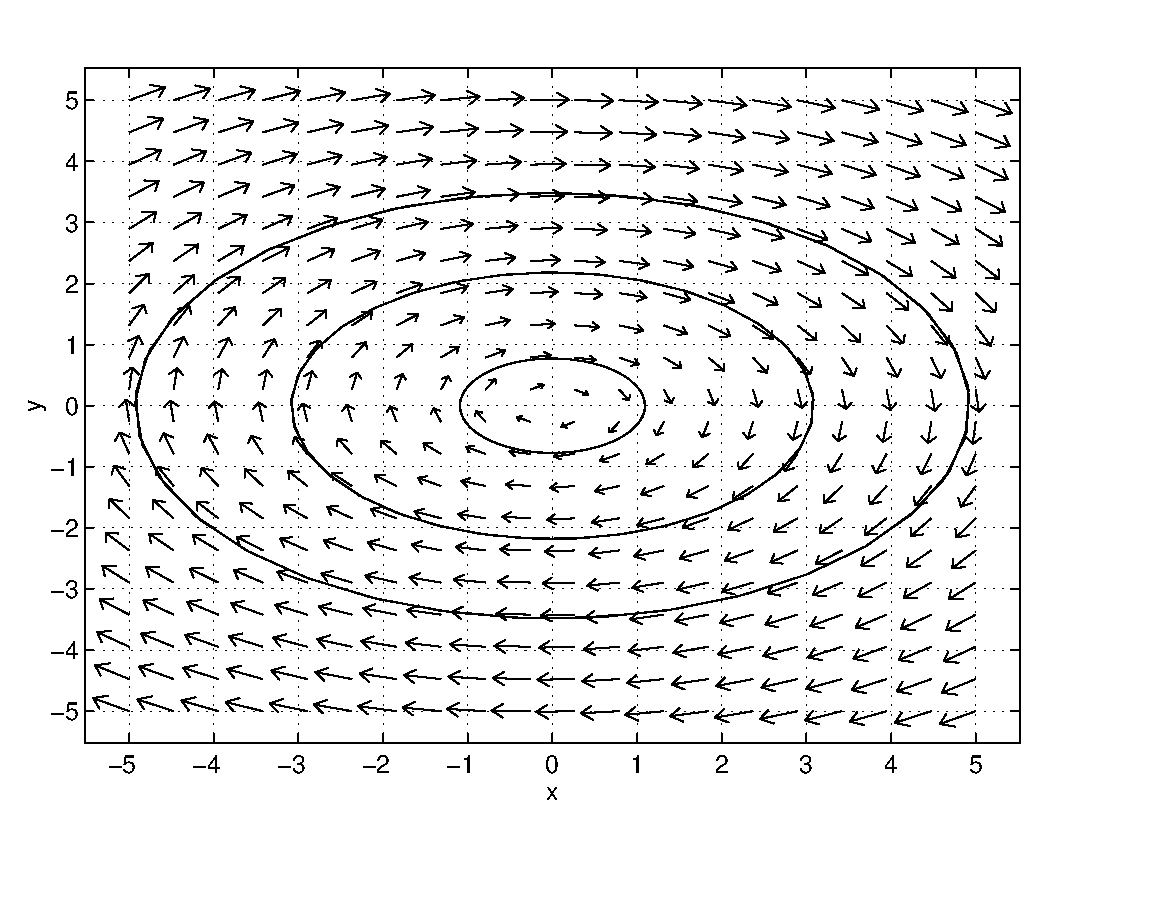
\psfig{file=exfigure/3-5-6a.eps,width=2.75in}
                       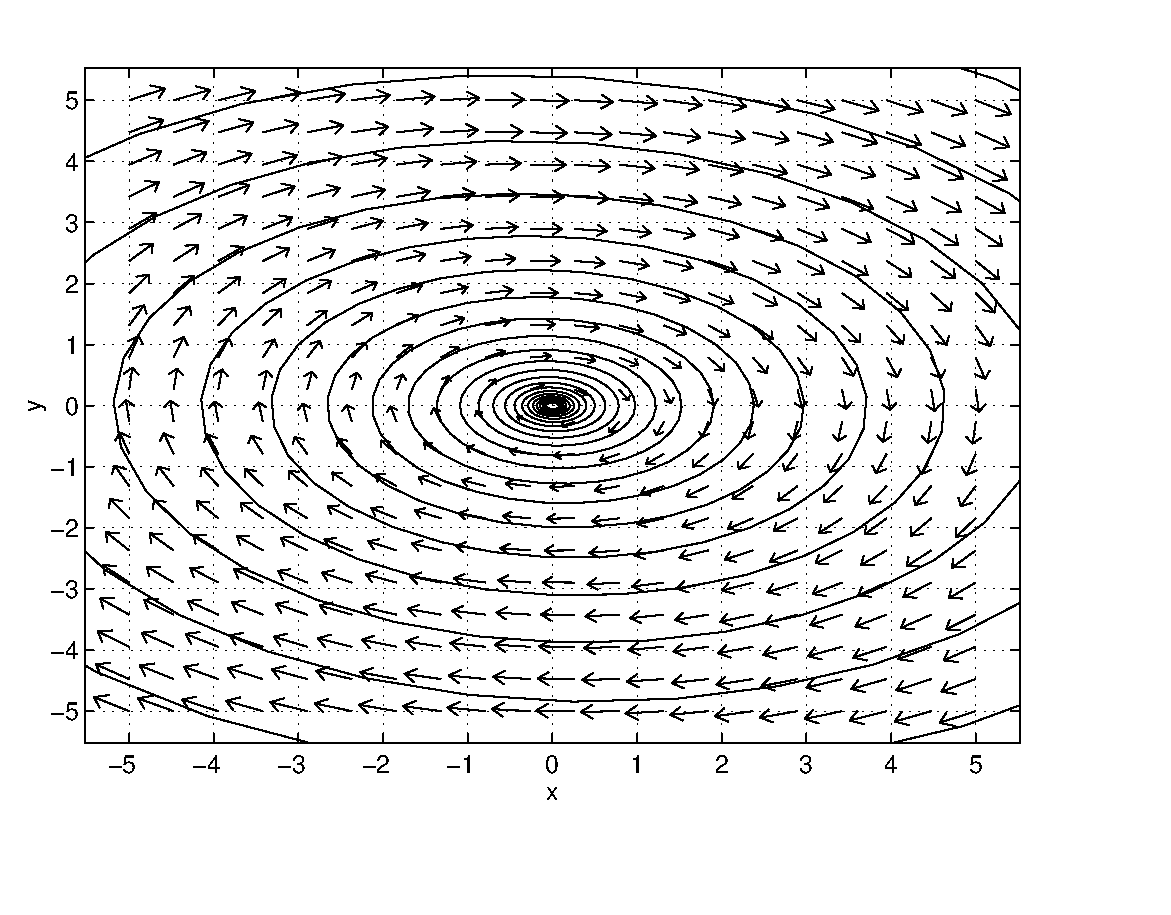
\psfig{file=exfigure/3-5-6b.eps,width=2.75in}}
			\exercaptwo{c6.9.2}
\end{figure}

\exer{E:PPa} \ans System $A$ has a spiral sink at the origin, $B$ has a
saddle, $C$ has a saddle node, and $D$ has an improper nodal source.

\soln Answers can be determined visually using the graphs and examples
from Sections~\ref{S:PlanarSystems} and \ref{S:6.9} of the text.

\exer{E:PPb} \ans The origin is asymptotically stable for $A$ and unstable
for $B$, $C$ and $D$.

\soln The origin is asymptotically stable if all solutions tend towards
the origin as $t \rightarrow \infty$.

\exer{E:PPc} \ans The traces of $A$, $B$ and $C$ are negative, and the
trace of $D$ is positive.

\soln The trace of a matrix is the sum of the eigenvalues, so the trace
is positive for sources, which have two positive eigenvalues and
negative for sinks, which have two negative eigenvalues.  The trajectories
of $C$ approach the eigenvector of $0$ as $t$ increases, rather
than tending away from it, so the nonzero eigenvector is negative and,
therefore, the trace is also negative.

\exer{E:PPd} \ans The determinants of $A$ and $D$ are positive, the
determinant of $B$ is negative, and the determinant of $C$ is zero.

\soln The determinant of a matrix is the product of the eigenvectors.  The
eigenvectors of $A$ are complex conjugates, so their product
is positive.  A saddle has one negative and one positive eigenvector, so
the determinant of $B$ is negative.  A saddle node has one zero
eigenvector, so the product of the eigenvectors of $C$ is zero.  An
improper nodal source has equal positive eigenvectors, so the determinant
of $D$ is positive.

\exer{E:PPe} \ans The discriminant of $A$ is negative, the discriminants of
$B$ and $C$ are positive, and the discriminant of $D$ is zero.

\soln The discriminant of a matrix is negative when the eigenvalues are
a complex conjugate pair, positive when the eigenvalues are real, and
zero when the eigenvalues are equal.

\exer{E:PQa} \ans The origin is hyperbolic, and the equilibrium at the origin
is a spiral source.

\soln The trace and determinant of $C$ are both nonzero, so the origin
is hyperbolic.  Since $\det(C) = 3 > 0$ and $\trace(C) = 2 > 0$,
the equilibrium at the origin is a source.  Since the discriminant
$D \equiv \trace(C)^2 - 4\det(C) = -8 < 0$, the origin is a spiral.

\exer{E:PQb} \ans The origin is hyperbolic, and the equilibrium at the origin
is a spiral source.

\soln The trace and determinant of $C$ are both nonzero, so the origin
is hyperbolic.  Since $\det(C) = 2 > 0$ and $\trace(C) = 2 > 0$,
the equilibrium at the origin is a source.  Since the discriminant
$D \equiv \trace(C)^2 - 4\det(C) = -4 < 0$, the origin is a spiral.

\exer{E:PQc} \ans The origin is hyperbolic, and the equilibrium at the origin
is an improper nodal source.

\soln The trace and determinant of $C$ are both nonzero, so the origin
is hyperbolic.  Since $\det(C) = 4 > 0$ and $\trace(C) = 4 > 0$,
the equilibrium at the origin is a source.  Since the discriminant
$D \equiv \trace(C)^2 - 4\det(C) = 0$, the eigenvalues of $C$ are equal.
Since $C$ is not a multiple of $I_2$, $C$ has only one eigenvector, so
the origin is an improper node.

\exer{E:PQd} \ans The origin is not hyperbolic, and the equilibrium at
the origin is a saddle node.

\soln The determinant of $C$ is zero, so the origin is not hyperbolic.
Since $\trace(C) = 2 \neq 0$, $C$ has one zero eigenvalue and one
nonzero eigenvalue, so the equilibrium at the origin is a saddle node.

\exer{E:PQe} \ans The origin is not hyperbolic, and the equilibrium at
the origin is a center.

\soln Since $\det(C) = 4 > 0$ and $\trace(C) = 0$, the origin is not
hyperbolic and $C$ has purely imaginary eigenvalues.  Thus, the
equilibrium at the origin is a center.

\exer{E:PQf} \ans The origin is not hyperbolic, and the equilibrium at
the origin is a shear.

\soln The trace and determinant of $C$ are both zero, so the origin
is not hyperbolic.  Since $C$ is not the zero matrix, the equilibrium
at the origin is a shear.

\exer{E:PQg} \ans The origin is hyperbolic, and the equilibrium at the origin
is a saddle.

\soln The trace and determinant of $C$ are both nonzero, so the origin
is hyperbolic.  Since $\det(C) = -3 < 0$, the equilibrium at the origin 
is a saddle.

\exer{E:notcircles}
By definition, a system $\dot{X} = CX$ is a center if the eigenvalues
of $C$ are purely imaginary.  This occurs when $\det(C) > 0$ and
$\trace(C) = 0$.  In this case, $\det(C) = 6$ and $\trace(C) = 0$, so
the system is indeed a center.  The phase portrait is shown in
Figure~\ref{E:notcircles}.  In this phase portrait and in the one
shown in Figure~\ref{F:center}, all
trajectories are closed ellipses.  However, the trajectories in
Figure~\ref{F:center} are circular, while the ones in this exercise
are not.  This is true because Figure~\ref{F:center} graphs the system
$\dot{X} = BX$, where
\[ B = \mattwo{0}{-\tau}{\tau}{0}, \]
while this problem graphs the system $\dot{X} = CX$, where $C = 
PBP^{-1}$ and $P \neq I_2$.

\begin{figure}[htb]
                       \centerline{%
                       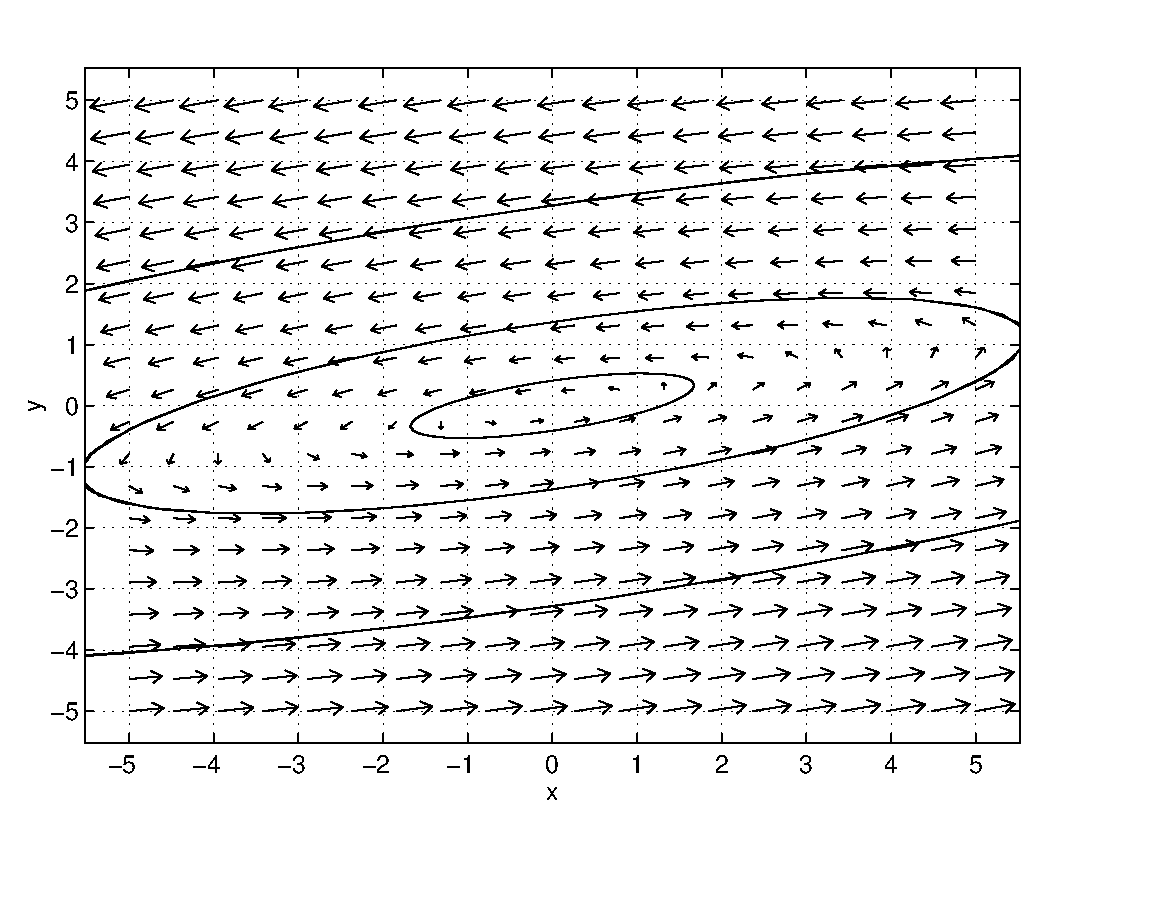
\psfig{file=exfigure/notcircles.eps,width=3.0in}}
                \exercap{E:notcircles}
\end{figure}

\exer{c6.9.5}
By definition, a system $\dot{X} = CX$ is a shear if the system has two
zero eigenvalues.  In this case, $\det(C) = 0$ and $\trace(C) = 0$, so
the eigenvalues are $\lambda_1 = \lambda_2 = 0$.  The phase portrait of
this system is shown in Figure~\ref{c6.9.5}a, and the phase portrait of
\Ref{e:00} is shown in Figure~\ref{c6.9.5}b.  In both phase portraits,
all trajectories are straight lines parallel to the eigenvector.  However,
in \ref{c6.9.5}b, the trajectories are parallel to the $x$-axis, whereas
in \ref{c6.9.5}a, they are not.

\begin{figure}[htb]
                       \centerline{%
                       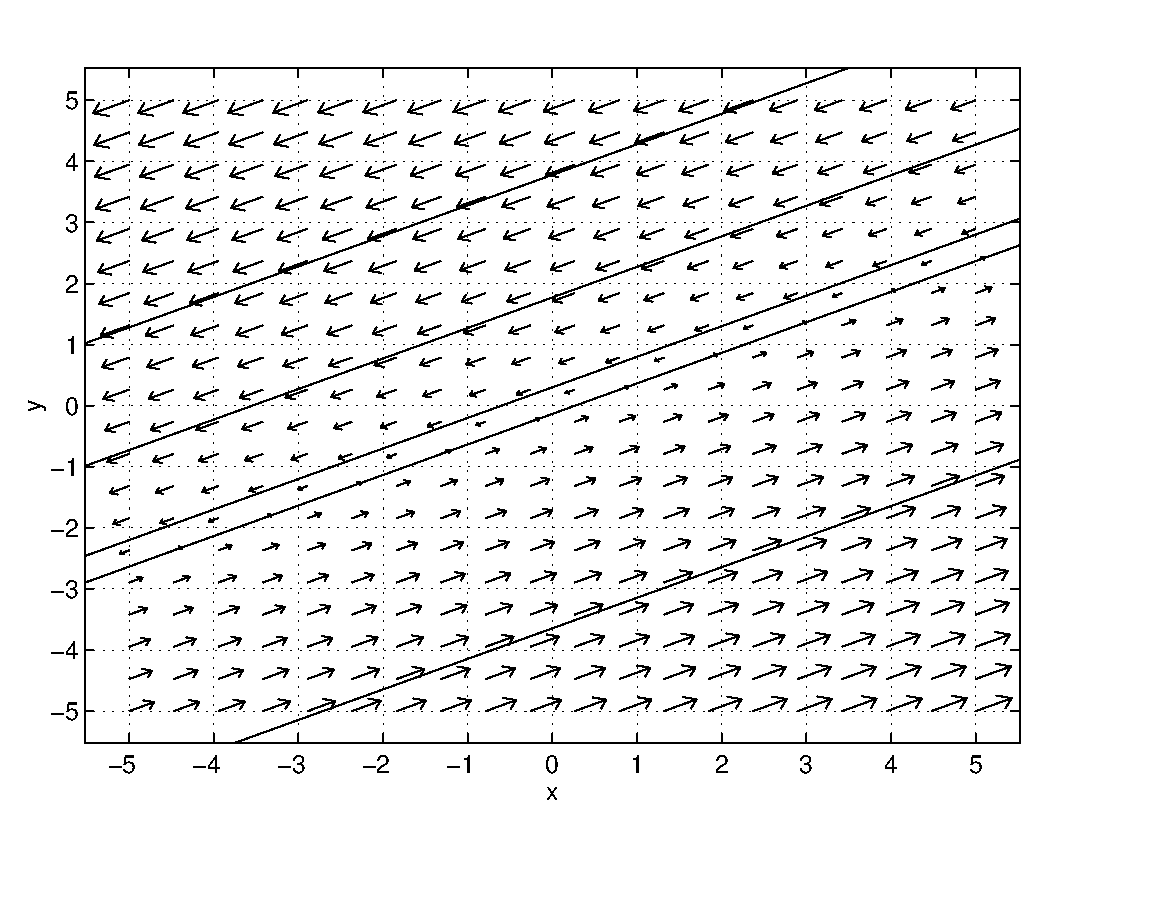
\psfig{file=exfigure/6-9-5a.eps,width=2.75in}
                       \psfig{file=exfigure/6-9-5b.eps,width=2.75in}}
                \exercaptwo{c6.9.5}
\end{figure}





\end{document}
